\documentclass[11pt,a4paper]{article}
\usepackage[T1]{fontenc}\usepackage{lmodern}
\usepackage[margin=22mm,headheight=14pt]{geometry}
\usepackage{amsmath,amssymb,bm,booktabs,tabularx,array,graphicx,float,fancyhdr,microtype,xcolor}
\usepackage[colorlinks=true,linkcolor=blue!45!black,urlcolor=blue!45!black,citecolor=blue!45!black]{hyperref}
\setlength{\parindent}{0pt}\setlength{\parskip}{5pt}\renewcommand{\arraystretch}{1.15}
\pagestyle{fancy}\fancyhf{}\fancyhead[L]{\small QFT Project B | Step 10}\fancyhead[R]{\small Group B}\fancyfoot[C]{\thepage}
\newcommand{\dd}{\mathrm{d}}
\begin{document}\hypersetup{pageanchor=false}
\begin{titlepage}\centering\vspace*{3mm}

\includegraphics[width=36mm]{assets/bits_logo.png}\par\vspace{13mm}
{\Large\bfseries BITS PILANI K.K. BIRLA GOA CAMPUS\par}\vspace{3mm}
{\large\bfseries Department of Physics\par}\vspace{18mm}
{\LARGE\bfseries What Quantum Trace Can\\[2mm] a Heavy Particle Leave?\par}\vspace{6mm}
{\large Curvature--Spectator Entanglement\\and the Cosmological Collider\par}\vspace{10mm}
{\large\bfseries Step 10: Entropy--Signal Comparison\par}\vspace{17mm}
{\Large\bfseries Group-B\par}\vspace{5mm}
\begin{tabular}{ll}Priyansh Rawat & 2023B5A70968G\\Mayank Sinha & 2023B5A70942G\\Samarth Bhatnagar & 2023B5A70853G\end{tabular}
\vfill{\large Under Professor: Rudranil Basu\par}\vspace{7mm}{29 October 2026\par}
\end{titlepage}\setcounter{page}{1}\hypersetup{pageanchor=true}
\section{Comparison at a common evaluation time}
The Gaussian entropy belongs to the quadratic state, while the spectator bispectrum is calculated to first order in $\lambda_3$. We compare entropies and power at the common time $x=0.01$. A selected mass/mixing control evaluates $F$ at the same triangle $r=0.03$ after regulator extrapolation.
\begin{center}\small\begin{tabular}{lllll}\toprule $M$ & $g$ & $S_q$ (nats) & $\Delta P_q/P_{q,0}$ & $F(0.03)$\\\midrule
$2$ & $0.05$ & $5.094\times10^{-5}$ & $9.297\times10^{-4}$ & $-5.084\times10^{-11}$\\
$2$ & $0.1$ & $1.846\times10^{-4}$ & $0.003714$ & $-3.986\times10^{-10}$\\
$2$ & $0.2$ & $6.790\times10^{-4}$ & $0.01478$ & $-2.936\times10^{-9}$\\
$1.8$ & $0.1$ & $0.001377$ & $0.005765$ & $3.916\times10^{-11}$\\
$2.4$ & $0.1$ & $7.630\times10^{-5}$ & $0.001825$ & $4.488\times10^{-11}$\\\bottomrule\end{tabular}\end{center}\begin{figure}[H]\centering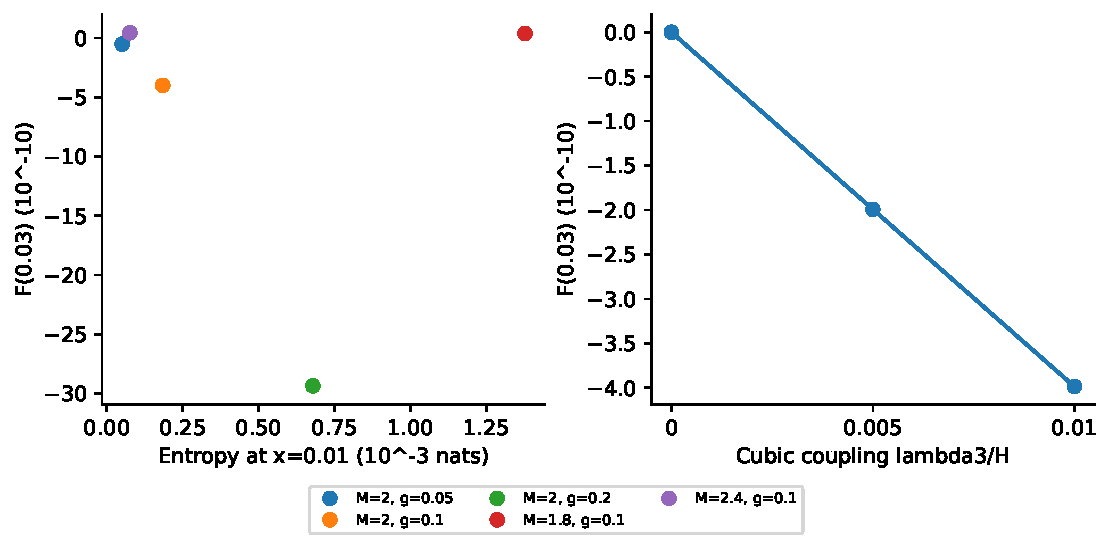
\includegraphics[width=.91\linewidth]{figures/entropy_signal_control.pdf}\caption{Selected entropy--signal points and the cubic-coupling control. A single-triangle value depends on oscillation phase as well as amplitude, so the left panel is not an entropy--clock-amplitude law.}\end{figure}The baseline entropy is $1.846\times10^{-4}$ nats per real sector. Comparing different masses at one triangle can change the signal sign through its phase. The full clock fit at the baseline point, rather than $F$ at a single $r$, is used for the mass assessment in Step 9.

\newpage
\section{Cubic control and recoverability}
At fixed $M=2$ and $g=0.1$, changing $\lambda_3$ does not alter the quadratic covariance. The leading bispectrum scales linearly:
\begin{center}\small\begin{tabular}{lll}\toprule $\lambda_3/H$ & $S_q$ & $F(0.03)$\\\midrule
$0$ & $1.846\times10^{-4}$ & $0$\\
$0.005$ & $1.846\times10^{-4}$ & $-1.993\times10^{-10}$\\
$0.01$ & $1.846\times10^{-4}$ & $-3.986\times10^{-10}$\\\bottomrule\end{tabular}\end{center}
This is a direct counterexample to inferring the three-point amplitude from Gaussian entropy alone: the same entropy accompanies zero, half-strength and full-strength cubic signals. It does not establish the absence of correlations within a restricted fixed-coupling parameter family.
For an illustrative recoverability comparison we apply the same mock covariance $\Sigma=\sigma_F^2 I$ with $\sigma_F=10^{-10}$ to all three signals. For the fitted baseline clock template $t_i$, the matched-template ratio is $\sqrt{t^T\Sigma^{-1}t}$. The template and covariance are specified assumptions, not a survey forecast.
\begin{center}\small\begin{tabular}{ll}\toprule $\lambda_3/H$ & Known-template signal/noise\\\midrule
$0$ & $0$\\
$0.005$ & $49.81$\\
$0.01$ & $99.63$\\\bottomrule\end{tabular}\end{center}
The signal/noise ratio changes with the cubic coupling while the Gaussian entropy stays fixed. Giving each signal the same fractional noise instead would conceal this amplitude dependence.
The core project now includes the analytic single-field reference, validated Gaussian entropy map, analytic in-in test, converged baseline spectator signal and an explicit mass-fit stability assessment. Larger clock-amplitude scans over masses and mixings remain extensions. These calculations concern the specified fields and state; they do not constitute a cosmological Bell test or an observational detection.\begin{thebibliography}{9}\small
\bibitem{gaussian} C. Weedbrook et al., \emph{Gaussian Quantum Information}, Rev. Mod. Phys. 84, 621 (2012), \href{https://arxiv.org/abs/1110.3234}{arXiv:1110.3234}.
\bibitem{chen} X. Chen and Y. Wang, \emph{Quasi-Single Field Inflation and Non-Gaussianities}, JCAP 04 (2010) 027, \href{https://arxiv.org/abs/0911.3380}{arXiv:0911.3380}.
\bibitem{collider} N. Arkani-Hamed and J. Maldacena, \emph{Cosmological Collider Physics}, \href{https://arxiv.org/abs/1503.08043}{arXiv:1503.08043}.\end{thebibliography}
\textbf{Code and supporting data:} \href{https://github.com/rawatpriyansh17/QFT-PROJECT-GROUP-B/tree/main/step10}{step10 on GitHub}.\newpage\section*{Contributions (equal)}\begin{center}\begin{tabularx}{\linewidth}{p{33mm}X}\toprule Member & Contribution\\\midrule Priyansh Rawat & Entropy--signal comparison and conclusions.\\[3mm]Samarth Bhatnagar & Cubic-coupling and common-covariance controls.\\[3mm]Mayank Sinha & Selected parameter comparisons, numerical tables and figure.\\\bottomrule\end{tabularx}\end{center}\end{document}